\documentclass[11pt]{article}
\usepackage[utf8]{inputenc}
\usepackage[pdftex]{graphicx}
\usepackage{pdfpages}
\usepackage[english]{babel}
\usepackage [autostyle, english = american]{csquotes}
\usepackage{mathtools}
\usepackage{float}
\usepackage{xcolor}
\usepackage{listings}
\usepackage{fancyvrb}
\usepackage{caption,subcaption}
%\usepackage{subfigure}
\usepackage[margin=0.6in]{geometry}
\usepackage{adjustbox}
\usepackage{listings}
\usepackage{hyperref}
\usepackage{wrapfig}
\usepackage{newfloat}
\usepackage[cm]{fullpage}
\usepackage[cachedir=build,newfloat,outputdir=build]{minted}
\usepackage{verbatim}

\definecolor{mintedbackground}{rgb}{0,0,0}
\usemintedstyle{tango}
\newenvironment{code}{\captionsetup{type=listing}}{}
\SetupFloatingEnvironment{listing}{name=Source Code}
\captionsetup[subfigure]{subrefformat=simple,labelformat=simple}
\renewcommand{\thelisting}{\arabic{listing}}
\renewcommand\thesubfigure{(\alph{subfigure})}
\definecolor{lightgray}{rgb}{.7,.7,.7}
\definecolor{gray}{rgb}{.4,.4,.4}
\definecolor{darkblue}{rgb}{0,0,.3}
\definecolor{gray}{rgb}{0.4,0.4,0.4}
\definecolor{darkblue}{rgb}{0.0,0.0,0.6}
\definecolor{cyan}{rgb}{0.0,0.6,0.6}
\renewcommand{\thelisting}{\arabic{listing}}
\renewcommand\thesubfigure{(\alph{subfigure})}

\definecolor{termback}{HTML}{DBE0E0}
\definecolor{termkeyword}{HTML}{50DA8B}
\lstdefinestyle{Bash}
{language=bash,
keywordstyle=\color{termkeyword},
basicstyle=\ttfamily,
morekeywords={@.},
alsoletter={:~\$.},
morekeywords=[2]{peter@kbpet:},
keywordstyle=[2]{\color{termkeyword}},
literate={\$}{{\textcolor{termkeyword}{\$}}}1 
         {:}{{\textcolor{termkeyword}{:}}}1
         {~}{{\textcolor{termkeyword}{\textasciitilde}}}1,
}

\geometry{
 a4paper,
 total={170mm,257mm},
 left=10mm,
 right=10mm,
 top=10mm,
 bottom=15mm
}
\graphicspath{ {images/} }

\lstset{
  basicstyle=\ttfamily,
  columns=fullflexible,
  showstringspaces=false,
  commentstyle=\color{gray}\upshape
}

\hypersetup{
    colorlinks,
    citecolor=black,
    filecolor=black,
    linkcolor=black,
    urlcolor=blue
}
 \newmintedfile[pycode]{python3}{
frame=lines,
framesep=2mm,
fontsize=\footnotesize,
showtabs =false,
autogobble=true,
breaklines=true,
mathescape=true
}
 \newmintedfile[shellcode]{bash}{
frame=lines,
framesep=2mm,
fontsize=\footnotesize,
showtabs =false,
autogobble=true,
breaklines=true,
mathescape=true
}

\newmintedfile[rcode]{S}{
frame=lines,
framesep=2mm,
fontsize=\footnotesize,
showtabs =false,
autogobble=true,
breaklines=true,
mathescape=true
}
\newmintinline[ibash]{bash} {
}

\newmintinline[ipy]{python3} {
}
\RecustomVerbatimCommand{\VerbatimInput}{VerbatimInput}%
{fontsize=\footnotesize,
 %
 frame=lines,  % top and bottom rule only
 framesep=2em, % separation between frame and text
 %
 labelposition=topline,
 %
 commandchars=\|\(\), % escape character and argument delimiters for
                      % commands within the verbatim
 commentchar=*        % comment character
}

\newcommand*{\escape}[1]{\texttt{\textbackslash#1}}

\title{Assignment 4 \\ Introduction to Information Retrieval \\ CS734/834}
\author{John Berlin}
\date{\today}
\renewcommand\thesection{Q.\arabic{section}}
\renewcommand\thesubsection{\thesection}
\begin{document}
\maketitle
\newpage
\section*{Note}

\indent During the course of this class I have found myself having to reusing code from previous assignments and re-working them for use in the current question I am working on at the time. This came to a head in this assignment where the changes to existing code became non-trivial which lead me to create more generalized versions of common operations used throughout this course. In order to keep the answers to questions about the methodology used in answering rather than implementation details using these generalized methods I will explain what they do here. The python3 classes seen in \autoref{code:cntx} are to be utilized with the context control statement \ipy{with} most commonly used with the \ipy{open} statement which opens a file object and automatically closes it when the control flow of the program exits that context. This is en-essence what each of these classes do. \newline   \newline  

The BeautifulSoupFromFile classes takes the path to a file plus the parser type used when creating the soup i.e html or xml and returns to the context using it the soup produced from opening the file and creating a new BeautifulSoup. AutoSaver and AutoSaveCsv takes the type to be save (python list or dictionary) with the path to the file to be written and returns to the calling context an empty version of the type specified to be populated in the scope of that context finally saving the types content to the file path when the context is exited. They also take optional arguments of functions which are used to format the output and or select what entities in they save type to be written to file. RunCommandSaveOut classes takes a function producing a \ipy{subprocess.Popopen} class, the command line arguments to pass to the function and supplies the function with a file object by which the standard output of the spawned process is serialized to. CleanFileLines class reads the contents of a specified file and applies a cleaning function to the contents (for example: $f(``A,B,C,X,Y,Z\escape{n}") \to ``A,B,C"$ ) returning to the context the cleaned lines with the option to save the cleaned lines back to the originating file. FileLinePrinter operates similarly but only prints the raw lines of the specified files. SelectFromFile also applies a transformation function to the files content but also applies a selector function to the cleaned contents of the file returning to the context only what is produced  after applying it to the files contents. RandFinderFile operates similarly but the selection function supplied is to randomly select a line from the files content which is then returned to the context.  \newline   \newline  

The other functions used in answering the questions in this assignment follow the convention of the previous assignments defining less intensive helpers in the file util.py seen in \autoref{code:util}.  Also the shell script created to run galago commands in assignment 3 \autoref{code:rungal} was also utilized with the eval argument which sets up the correct command line arguments to run the galago function eval as the  default options for this do not return results required for this assignment. It explicitly asks for all available metrics to be computed the full list of metrics can be seen in \autoref{code:rungal}. A more specialized utility file was created for use with the context classes described previously for use with the output of galago functions especially for sanatizing the output of the query runs to work with the eval function of galago. These functions can be seen in \autoref{code:cacm_help}.  \newline \newline Finally it must also be noted that I will be using an updated version of galago (v3.10) in this report. For a more detailed explanation as to why and the differences in this version from the one used by the textbook please consult this same section in the report for assignment 3 for more details.
\newpage
\section{Question 8.3} \label{q1}
\begin{verbatim}
For one query in the CACM collection (provided at the book website), 
generate a ranking using Galago, and then calculate average precision, NDCG at 5
and 10, precision at 10, and the reciprocal rank by hand.
\end{verbatim}
\subsection{Answer} 
Like the previous assignments questions where galago was used to query a collection creation of the index and query creation is the first step. This process was automated thanks to the lessons learned from having used galago before and having the queries were supplied to us. Since the provided queries are in the old xml style they are converted to json after the index has been created.  The automation process can be seen in the python file \textbf{q1\_cacm\_query\_rel.py}, \autoref{code:q1} along with the rest of the code used in answering this question. Running the file \ibash{python3 q1_cacm_query_rel.py} for the first time will create the index, convert the queries and after the running the queries against the CACM collection execute the \textit{eval} function of galago against the runs results automatically. Subsequent executions of this file will not run the galago commands if the files produced by running this file are found to exist. The first time output generated can be seen in  \autoref{fig:cacmidx}.
\begin{figure}[H]
\centering
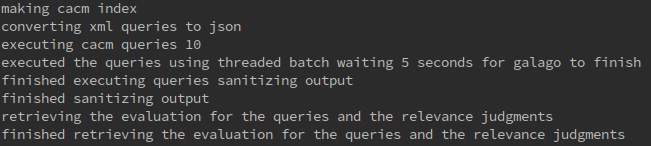
\includegraphics[scale=0.7]{q1buildidx.png}
\caption{Building CACM collection index}
\label{fig:cacmidx}
\end{figure}
Their is an extra step noted in the output generated by this python, \autoref{fig:cacmidx}, which is \textit{finished executing queries sanitizing output}. This extra step is required in order for the eval function of galago to work properly. The batch search function of galago as stated in the \href{https://sourceforge.net/p/lemur/wiki/Galago\%20Functions/}{documentation} produces output in the following format 
\begin{verbatim}
<qid> Q0 <docid> <rank> <score> <system-name> <begin> <end>
\end{verbatim}
Running the batch search command made the \textit{docid} part of the output contain the full path to a CACM document on my machine. The full path for the docid caused the \textbf{eval} function of galago to not produce any output. This puzzled me for upwards of thirty minutes as I attempted to figure out why by recreating the index and playing around with various parameters to the \textbf{batch-search} function. It was not until I looked at the provided \textit{cacm.rel} file provided on the textbooks webcite. \autoref{fig:cacmrel} shows the first few lines of this file.
\begin{figure}[H]
\centering
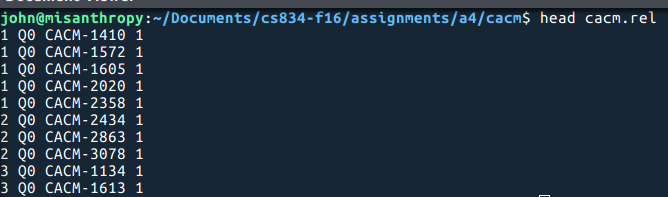
\includegraphics[scale=0.8]{camrell.png}
\caption{head cacm.rel}
\label{fig:cacmrel}
\end{figure}
As you can see in the output of running the unix command \textit{head} on the file there is only the name of the file contained in the collection with the query number it is relevant for and a weight (Q0 is disregarded by galago). On inspection I realized that galago must not be able to match a queries returned documents to the relevance file if they contain the full path to them. I could not find any option to suppress this in the output for the runs so cleaning the runs results to be in the form $<quid \ Q0 \ docid \ rank \ score>$  in order to be matched with the relevance file was the only way forward. After sanitizing the output the the relevance results for the run can was determined. Now the question stated \textbf{the reciprocal rank by hand} after a list of metrics to be calculated which could mean just the reciprocal rank or all of them but it also can be roughly coerced into the interpretation of by code utilizing values produced by code you wrote which is how I interpreted its meaning.  Plus I wanted to use a python file I found on gist a while back ;) which can be seen in \autoref{code:q1rnk}. \newline \newline
The query for the metrics calculation is selected by random from the runs results and then calculated by hand written code along with the output of the same metrics as galago computed them for a sanity check. The by hand calculation is done as following: select a random run from the batch-search runs \textit{eval} results output, select the relevant documents for that run from the \textit{cam.rel} file and  then select that runs returned documents from the batch-search output. If the run had relevant documents or the \textit{eval} results for query did not have NaN computed by galago for the metrics do the by hand computation of the metrics.  Queries 34 35 41 46 47 50 51 52 53 54 55 56 had NaN values for the metrics when calculated by galago\newline \newline
For each document returned by the query create a list of binary values indicated if the returned document at position $n$ was relevant (1) or not (0) then calculate NDCG@5 and NDCG@10, P@10, Average Precision using the created list plus the Reciprocal Rank. This process was done for three randomly chosen query 4 \autoref{fig:cam_rel4}, query 9 \autoref{fig:cam_rel9} and query 11 \autoref{fig:cam_rel11}, along with the galago computed scores for NDCG@5 and NDCG@10, P@10. It must be noted that galago computes Average Precision for MAP when consulting the source code to discover the available metrics. As seen in the figures the computed P@10 values for all three queries match the calculation done by galago while the NDCG values for queries 4 and 9 are way off in comparison to galago computed versions whereas query 11 had computed NDCG values off by only $.01$ for NDCG@5 and $.17$ for NDCG@10. Consulting the methods used to compute these metrics besides using numpy to calculate the score the methods for all intents and purposes are implemented correctly.  The number of returned documents for each each query was set to ten when executed using galago as the Google only 10 results per page in its search results.  As seen in the output queries 4,9 and 11 have 12, 9, and 19 relevant  documents respectfully according to the provided \textit{cam.rel} used in answering this question. This leads me to believe that galago is considering the full set of relevant documents in the calculations it returns. 
\begin{figure}[H]
\centering
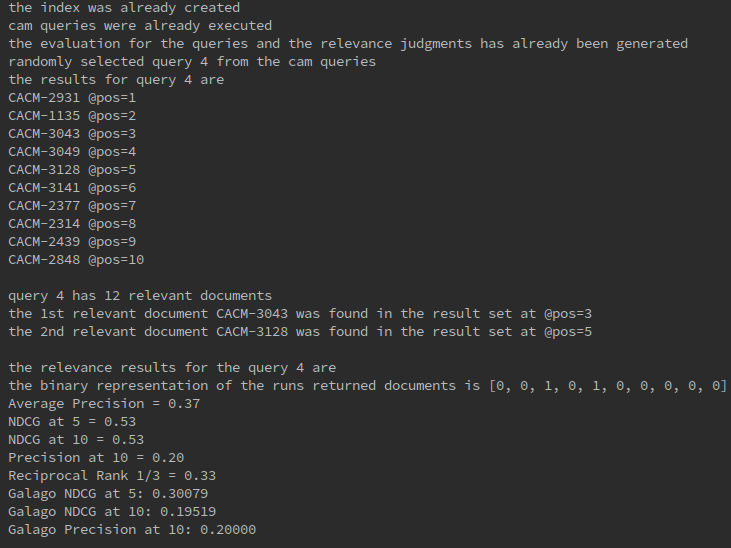
\includegraphics[scale=0.6]{q1run2.png}
\caption{Relevance Metrics For Queries 4}
\label{fig:cam_rel4}
\end{figure}

\begin{figure}[H]
\centering
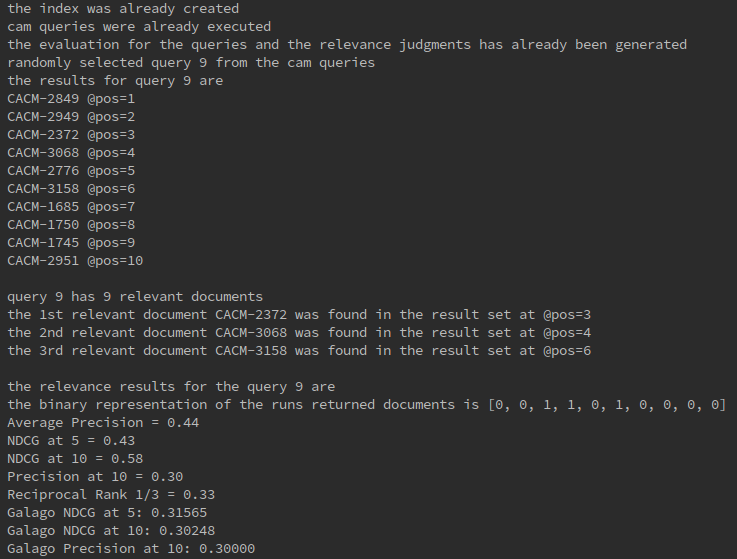
\includegraphics[scale=0.6]{q1_run3.png}
\caption{Relevance Metrics For Query 9}
\label{fig:cam_rel9}
\end{figure}
\begin{figure}[H]
\centering
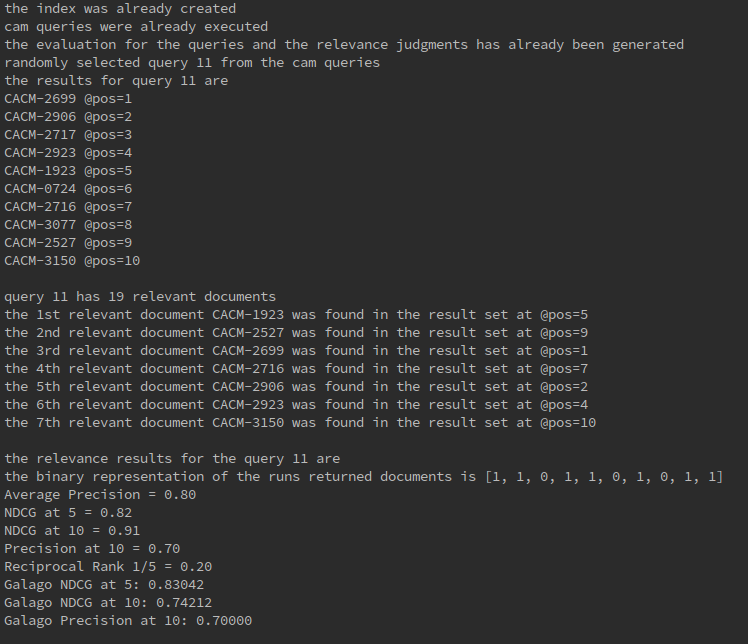
\includegraphics[scale=0.6]{q1run1.png}
\caption{Relevance Metrics For Query 11}
\label{fig:cam_rel11}
\end{figure}
\begin{code}
\captionof{listing}{Single CACM Query Relevance} 
\label{code:q1}
	\pycode{code/q1_cacm_query_rel.py}
\end{code}
\newpage
\section{Question 8.5} \label{q2}
\begin{verbatim}
Generate the mean average precision, recall-precision graph, average NDCG
at 5 and 10, and precision at 10 for the entire CACM query set
\end{verbatim}
\subsection{Answer} 
The values used in the graph for this question were retrieved from the results generated from \textit{eval} function used in \autoref{q1} and then saved to a csv file \autoref{code:q2py} for plotting via R \autoref{code:q2r}.  \autoref{fig:q2plot} shows the metrics plotted against each and it is clear to see that results follow a similar pattern. This plot also brings up the question of does galago consider the entire relevant document for a query in these calculations as was noted in \autoref{q1}. 
\begin{figure}[H]
\centering
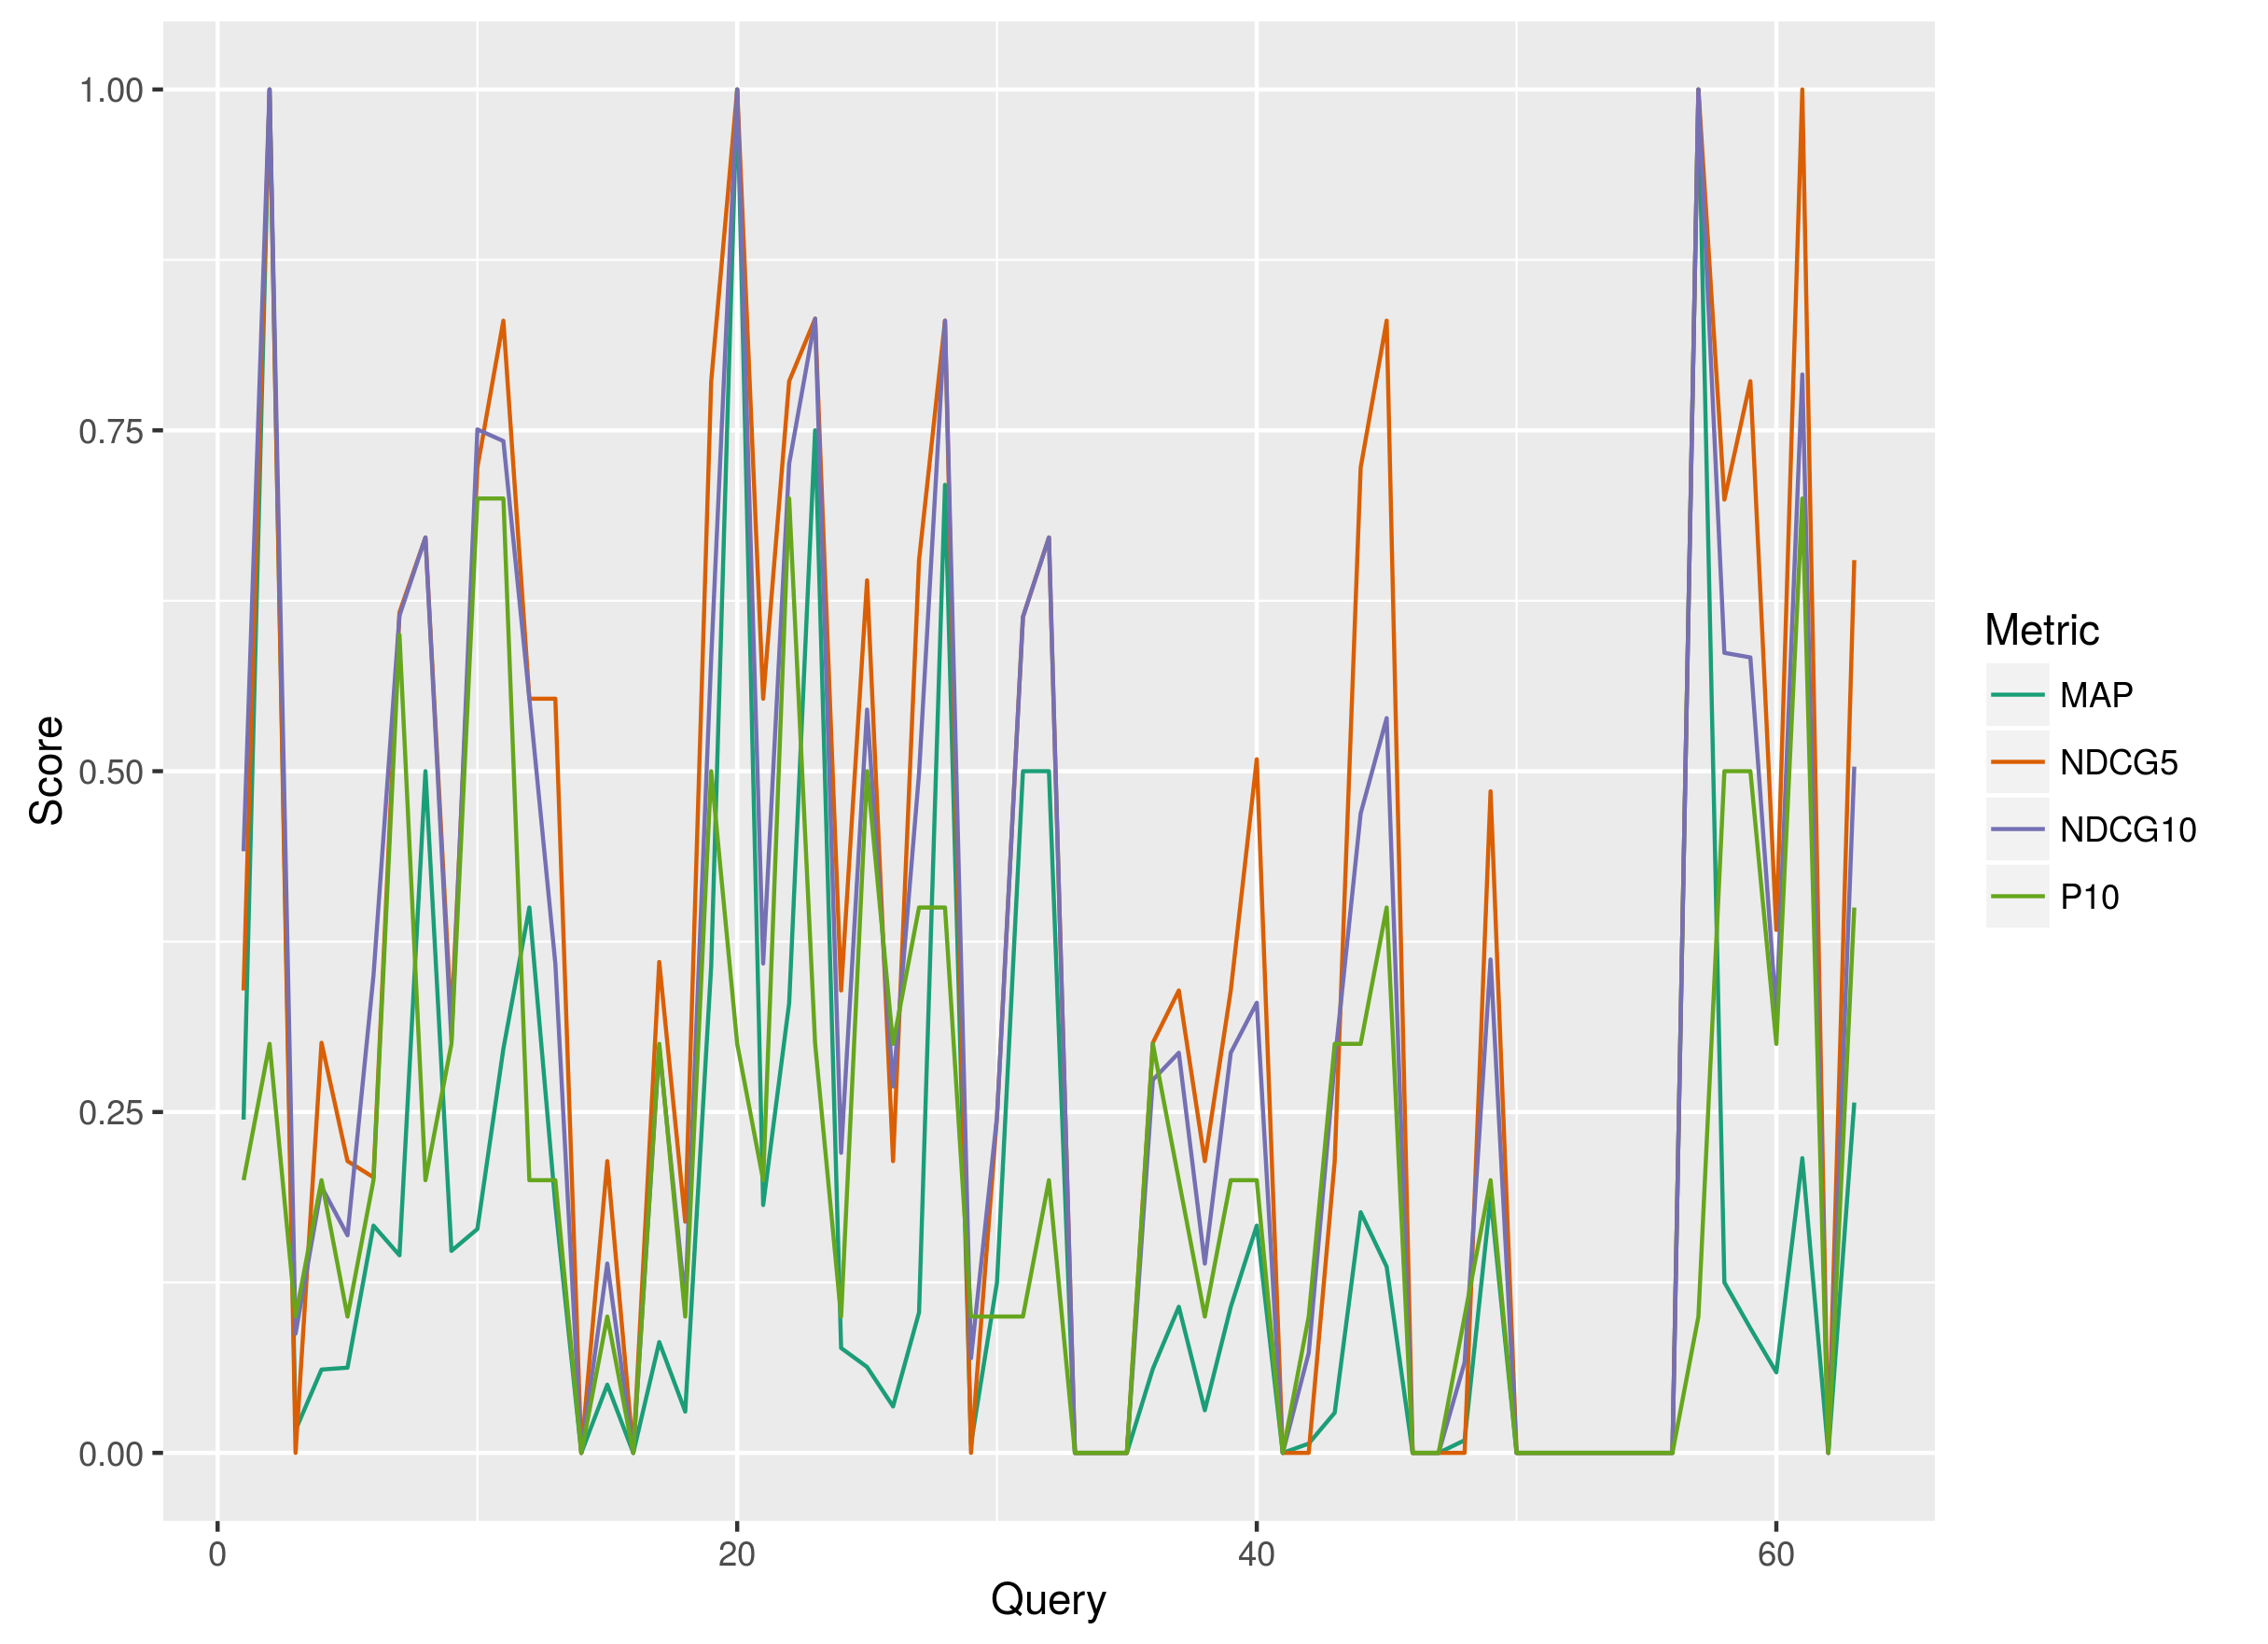
\includegraphics[scale=0.9]{q2_plot.png}
\caption{Galago Eval Metrics For All Queries}
\label{fig:q2plot}
\end{figure}
Considering \autoref{fig:q2plot2} which plots the Recall and Precision scores for each query as calculated by galago, they as well follow the pattern seen in \autoref{fig:q2plot}.
\begin{figure}[H]
\centering
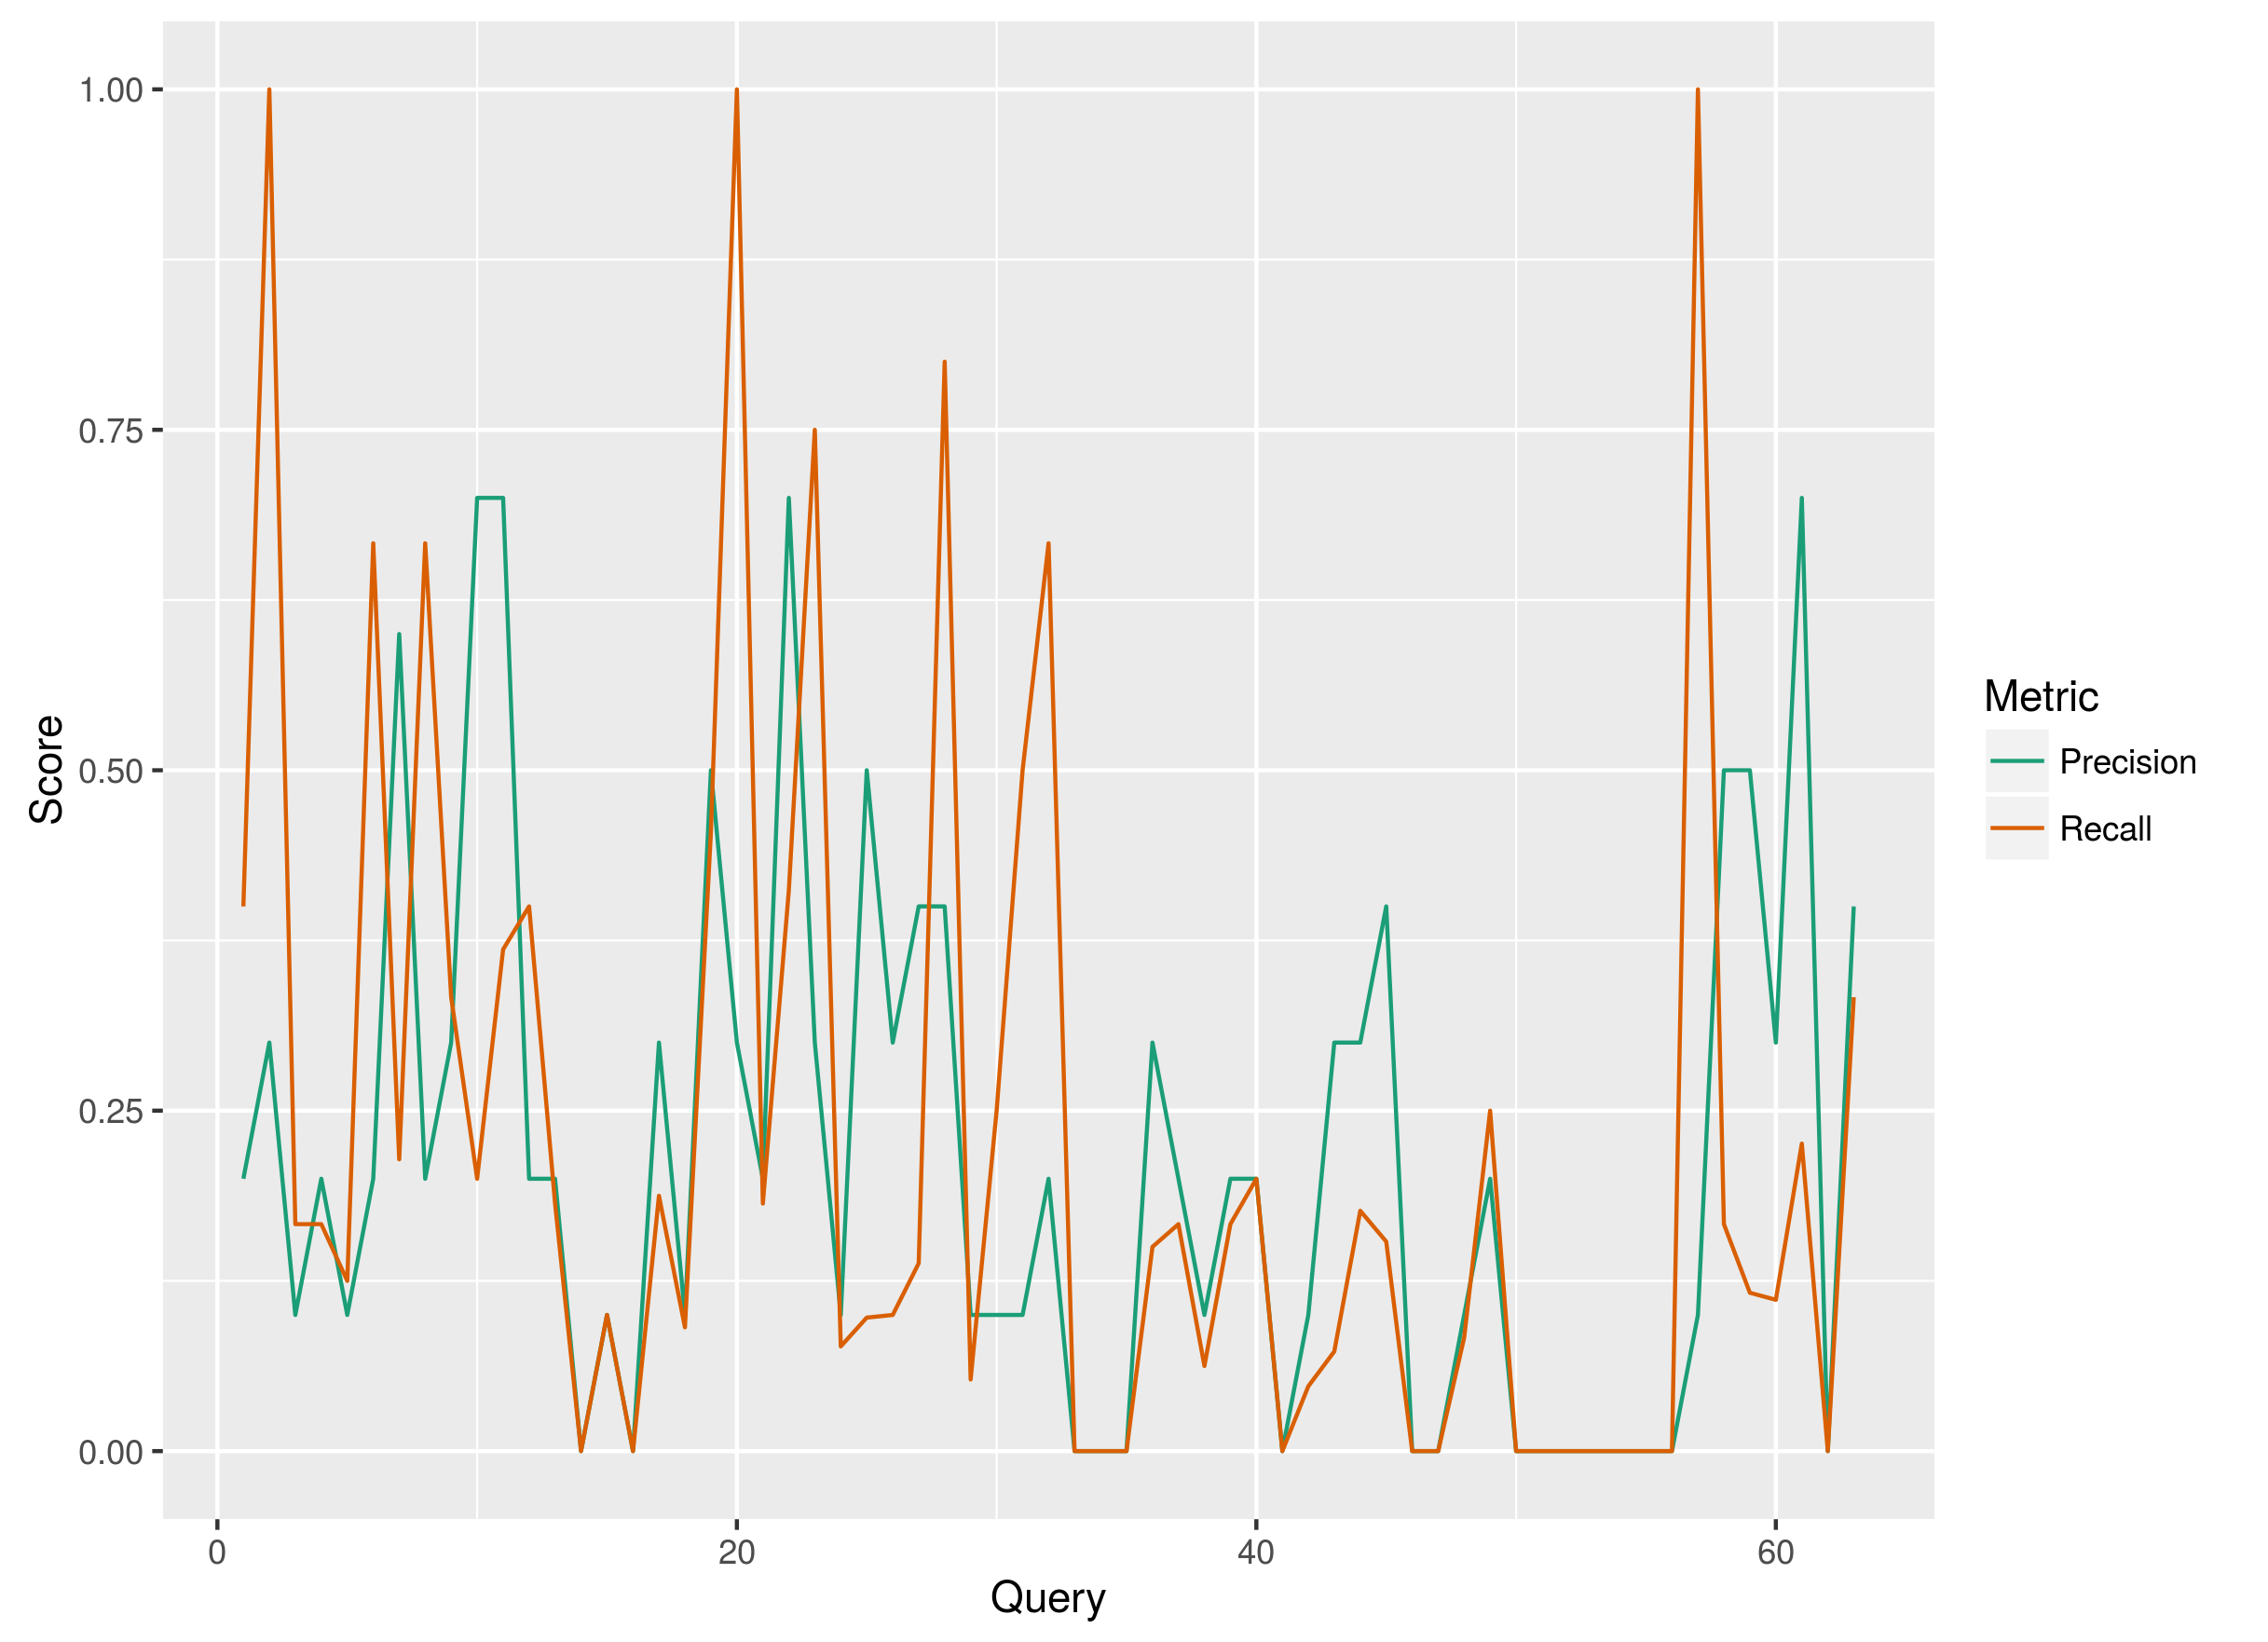
\includegraphics[scale=0.9]{q2_plot_rp.png}
\caption{Galago Eval Recall Precision For All Queries}
\label{fig:q2plot2}
\end{figure}
The seemingly eradicate hills and valleys are present in both plots and when considering \autoref{fig:q2plot2} it becomes clear that the overall performance of the queries was poor due to the number of queries with NaN values and how galago considers all relevant documents in its metrics.  Now consider \autoref{tbl:lt10} which shows the queries with less than 10 relevant documents and \autoref{fig:q2plot3} showing the number of relevant documents for the all of the CACM queries. \autoref{fig:q2plot3} shows a relatively similar pattern as is seen in \autoref{fig:q2plot} and \autoref{fig:q2plot2}.  \autoref{tbl:lt10} shows 19 out of 64 queries which had relevant document counts less than 10. These queries further confirm my assumption that galago considers all relevant documents as  \autoref{fig:q2plot} and  \autoref{fig:q2plot2} start out at 1.0 which is perfect. Then a sharp drop as query 2 only had 3 relevant documents and then back up for query 5 which had 8.
\begin{table}[ht]
\caption{Relevant Document $<$ 10 Count }
\begin{minipage}{.5\linewidth}
\centering
       \begin{tabular}{rr}
  \hline
 Query & Count \\ 
  \hline
 1 &   5 \\ 
2 &   3 \\ 
  3 &   6 \\ 
  5 &   8 \\ 
   6 &   3 \\ 
   8 &   3 \\ 
  9 &   9 \\ 
  12 &   5 \\ 
20 &   3 \\ 
   \hline
\end{tabular}
    \end{minipage}%
    \centering
    \begin{minipage}{.5\linewidth}
       \begin{tabular}{rr}
  \hline
 Query & Count \\ 
  \hline
23 &   4 \\ 
  28 &   5 \\ 
   30 &   4 \\ 
31 &   2 \\ 
  32 &   3 \\ 
  33 &   1 \\ 
  49 &   8 \\ 
  57 &   1 \\ 
   62 &   8 \\ 
  64 &   1 \\ 
   \hline
\end{tabular}
    \end{minipage} 
\label{tbl:lt10}
\end{table}

\begin{figure}[H]
\centering
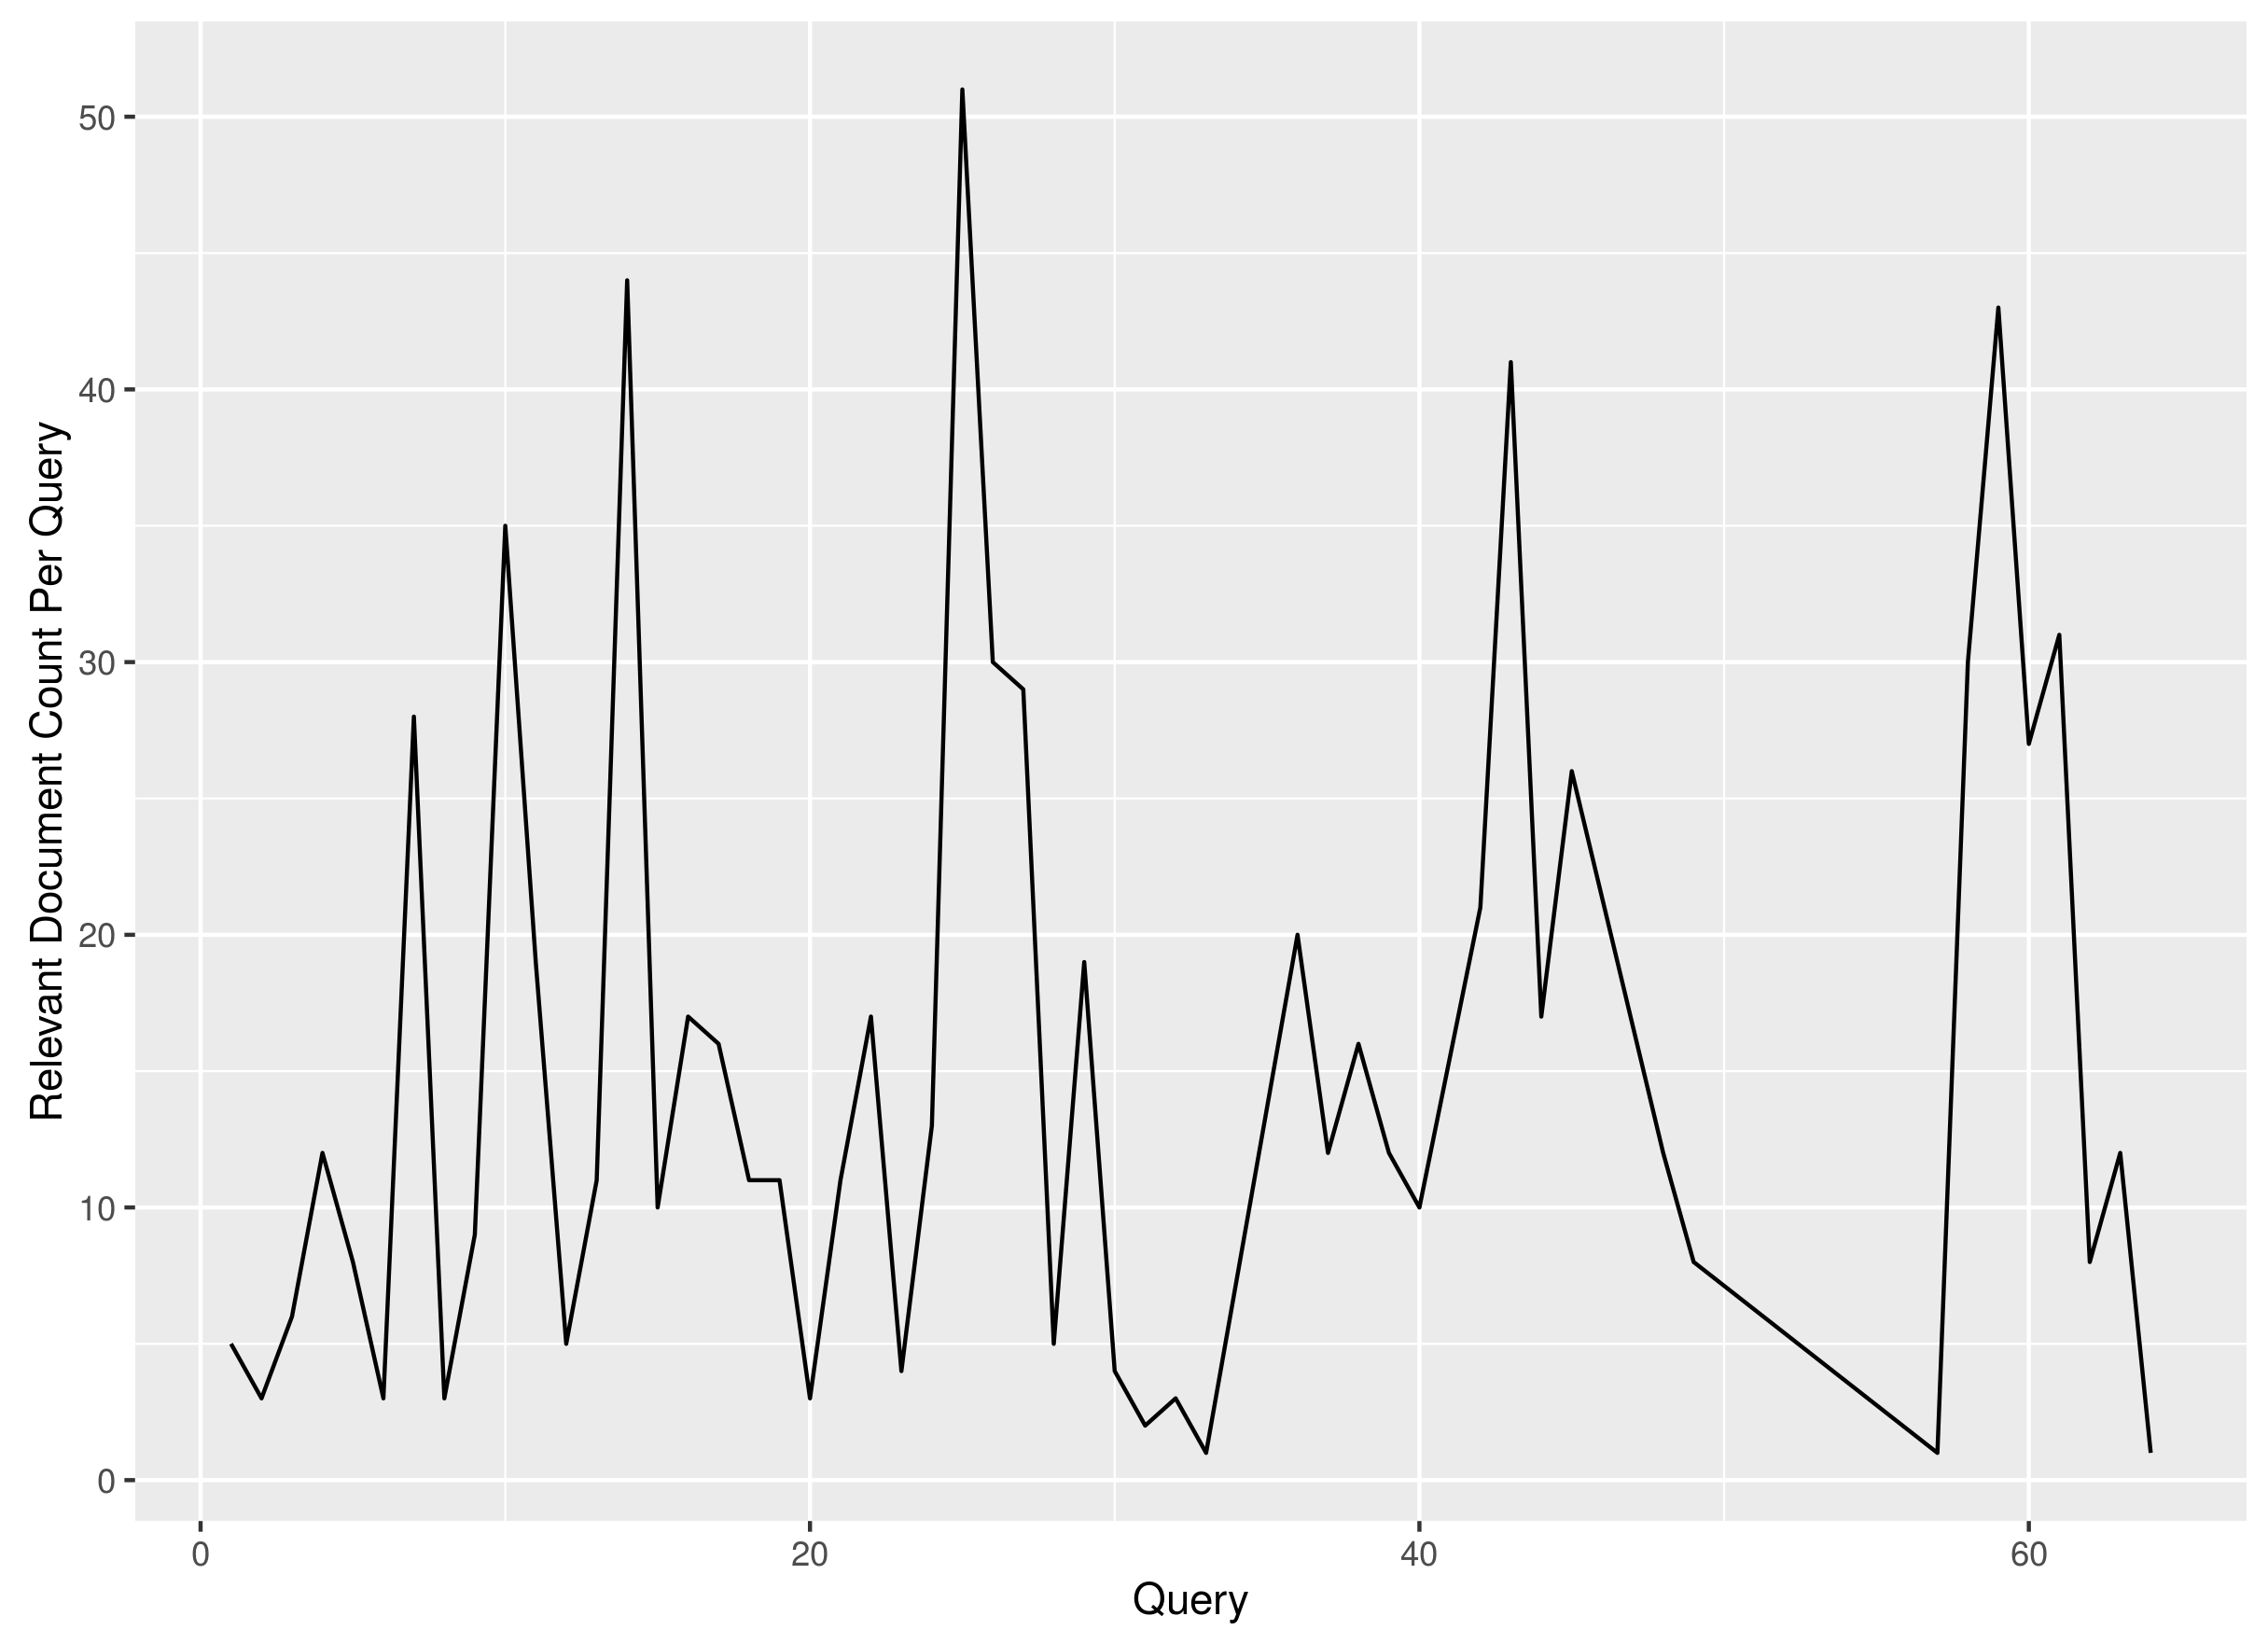
\includegraphics[scale=0.9]{q2_plot_rc.png}
\caption{Relevant Document Count For CACM Queries}
\label{fig:q2plot3}
\end{figure}
\begin{code}
\captionof{listing}{Graph Data File Generator} 
\label{code:q2py}
	\pycode{code/q2_8.5.py}
\end{code}
\begin{code}
\captionof{listing}{Graph Data File Generator Plotter} 
\label{code:q2r}
	\rcode{code/q2_plotter.R}
\end{code}
\newpage
\section{Question 8.7} \label{q3}
\begin{verbatim}
Another measure that has been used in a number of evaluations is R-precision.
This is defined as the precision at R documents, where R is the number of relevant
documents for a query. It is used in situations where there is a large variation in
the number of relevant documents per query. Calculate the average R-precision
for the CACM query set and compare it to the other measures.
\end{verbatim}
\subsection{Answer} 
Since galago computes the relevance metrics considering all relevant documents it is clear that the R-precision is one of the few metrics that would give an accurate results for all queries. This is due to it having the nice property of the R parameter which is the number of documents in the result set of a query which would be ten in this case.  The code used to generate the data and the graphs can be seen in \autoref{code:q3} and \autoref{code:q3p}. As a more in depth look at what would be causing the graph to behave as it does was done in \autoref{q2} my answer for this question will be more general. \autoref{fig:q3plot} shows the graph comparing R-Precision to the other metrics with loess smoothing applied in order to better compare these metrics. Also shown in this plot are all values for these metrics in the background in order to show the need for the smoothing as without it a comparison would be hard.  \newline \newline 
As was seen in the plots for \autoref{q2} the R-Precisions follows the same trend of dipping where the queries had below ten relevant documents or NaN values were computed. Unlike the other methods R-Precision appears to have less of a dramatic increase or decrease in its values. 
\begin{figure}[H]
\centering
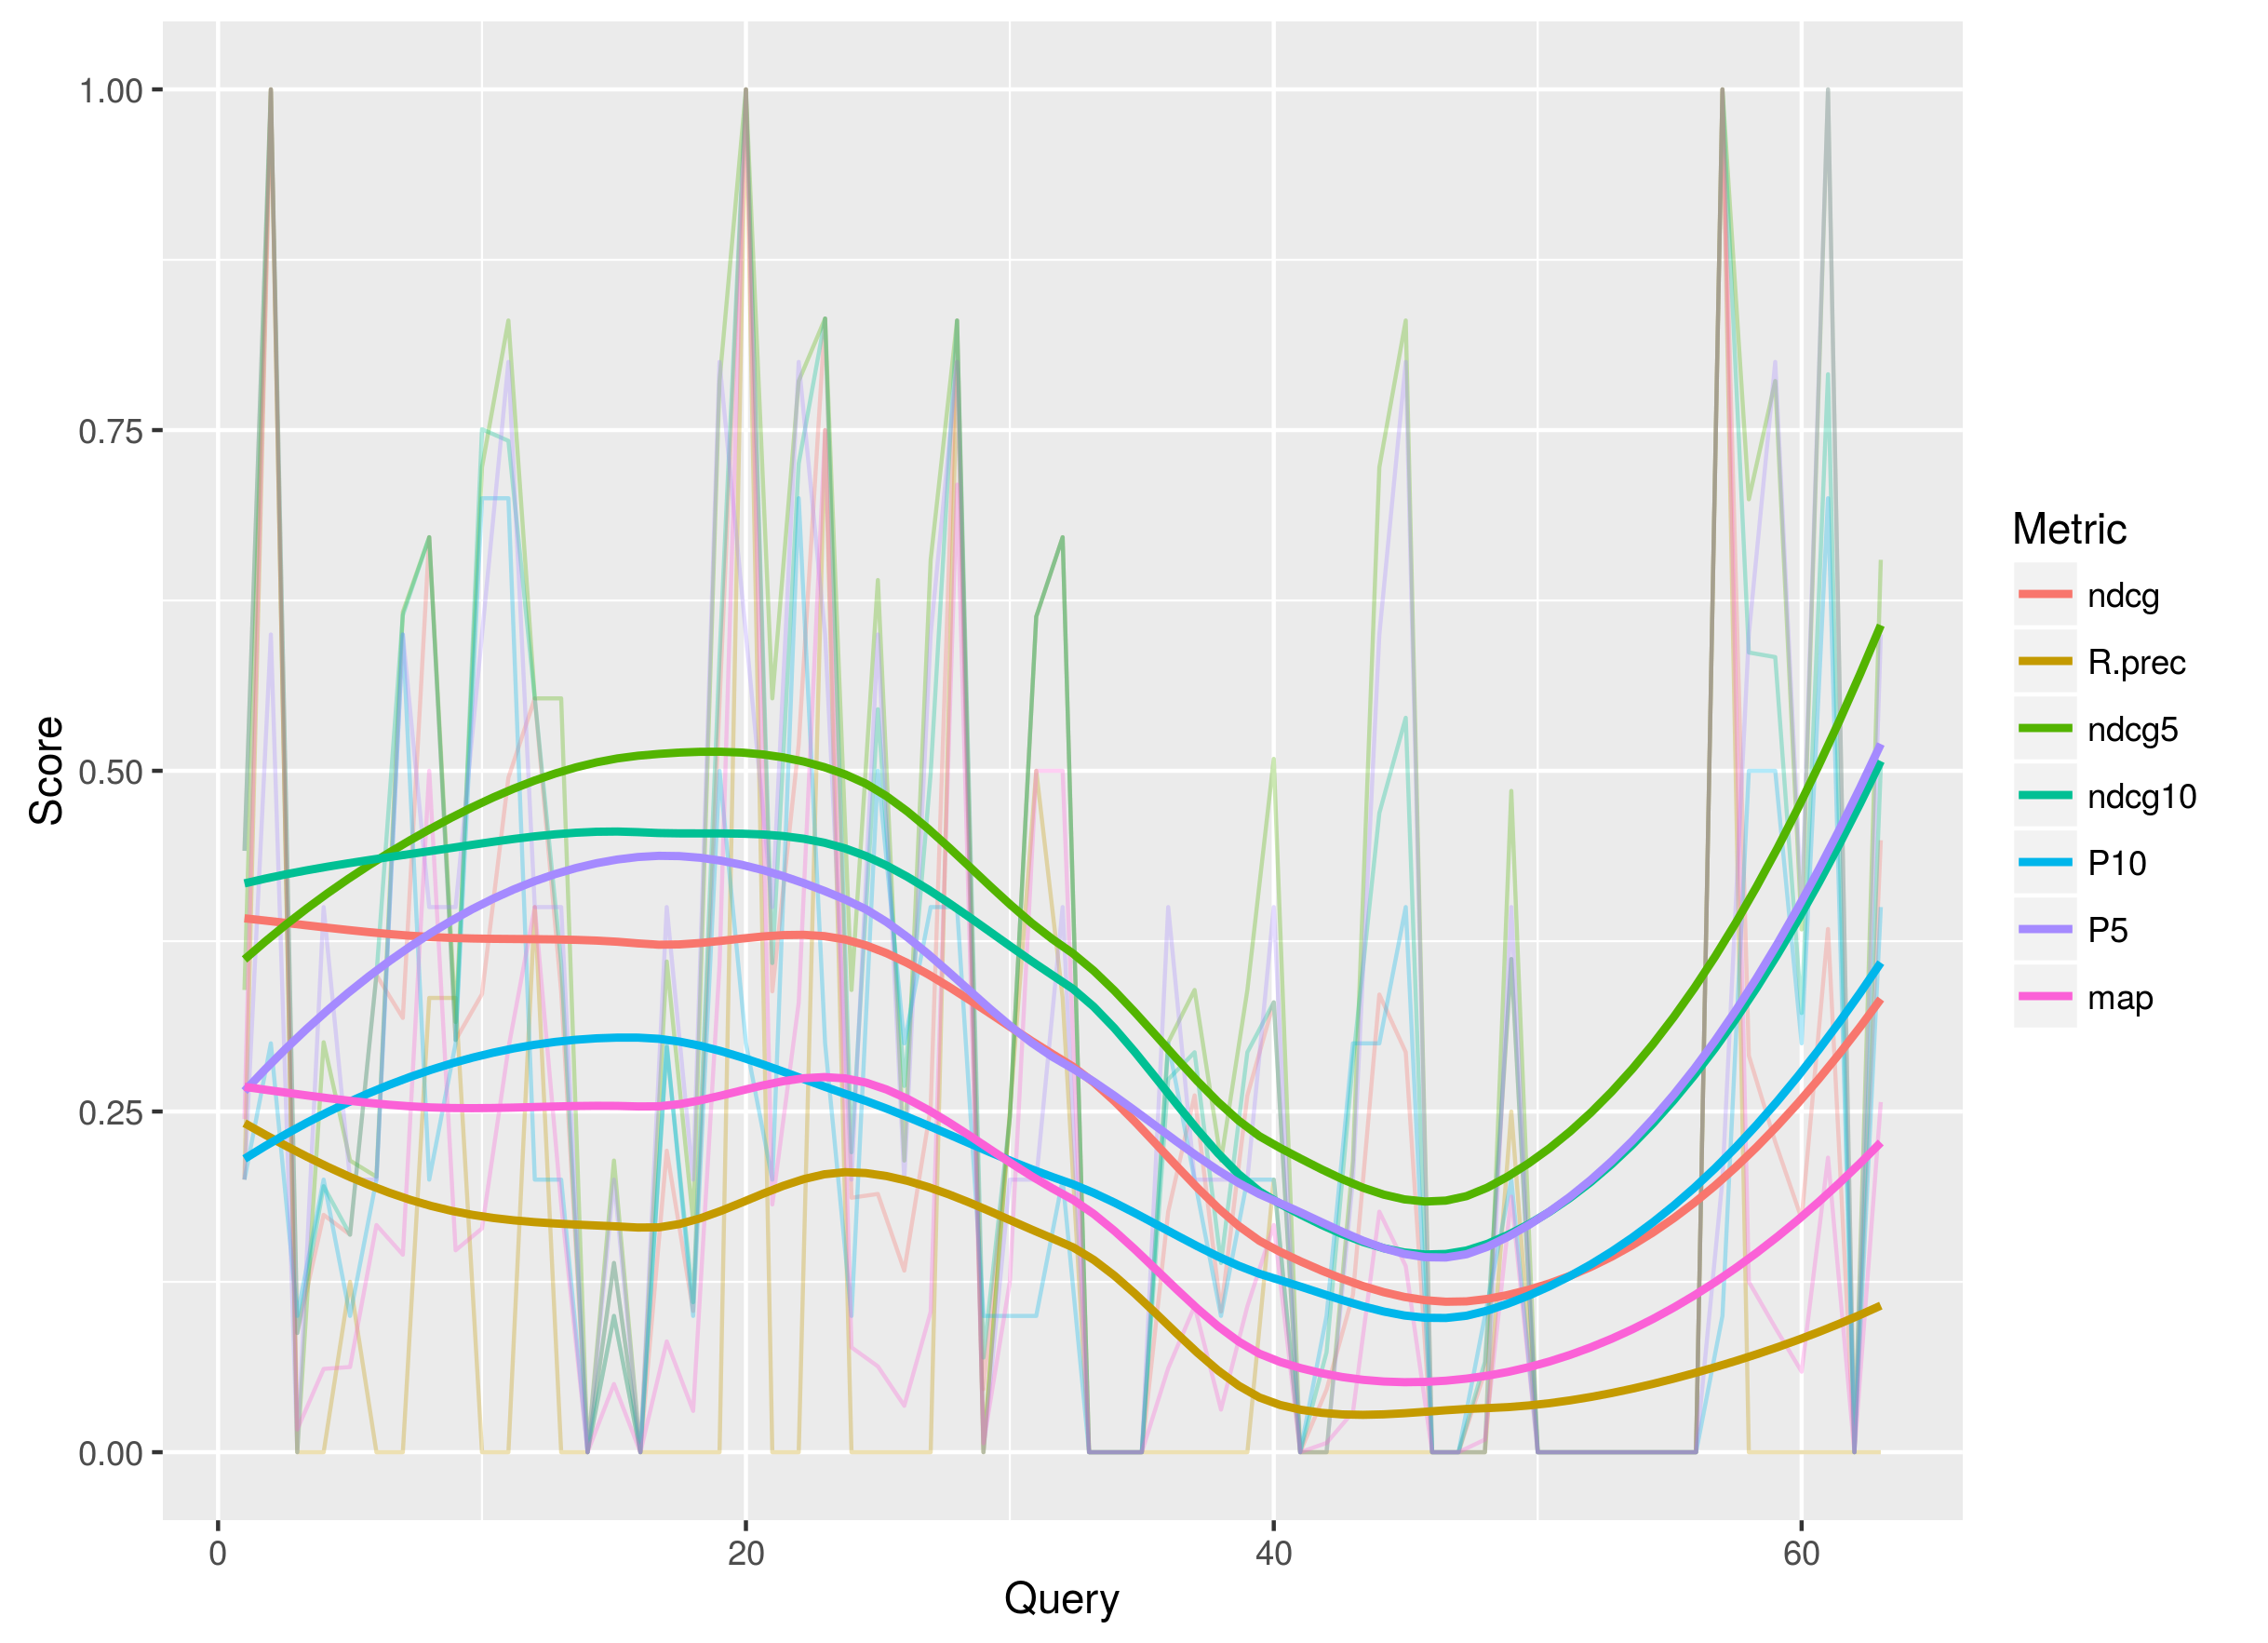
\includegraphics[scale=0.9]{q3_plot.png}
\caption{R-precision Comparison}
\label{fig:q3plot}
\end{figure}
Now to gain a better understanding of what is actually happening consider which show the r values at 20 and 100 respectively.
\begin{figure}[H]
\centering
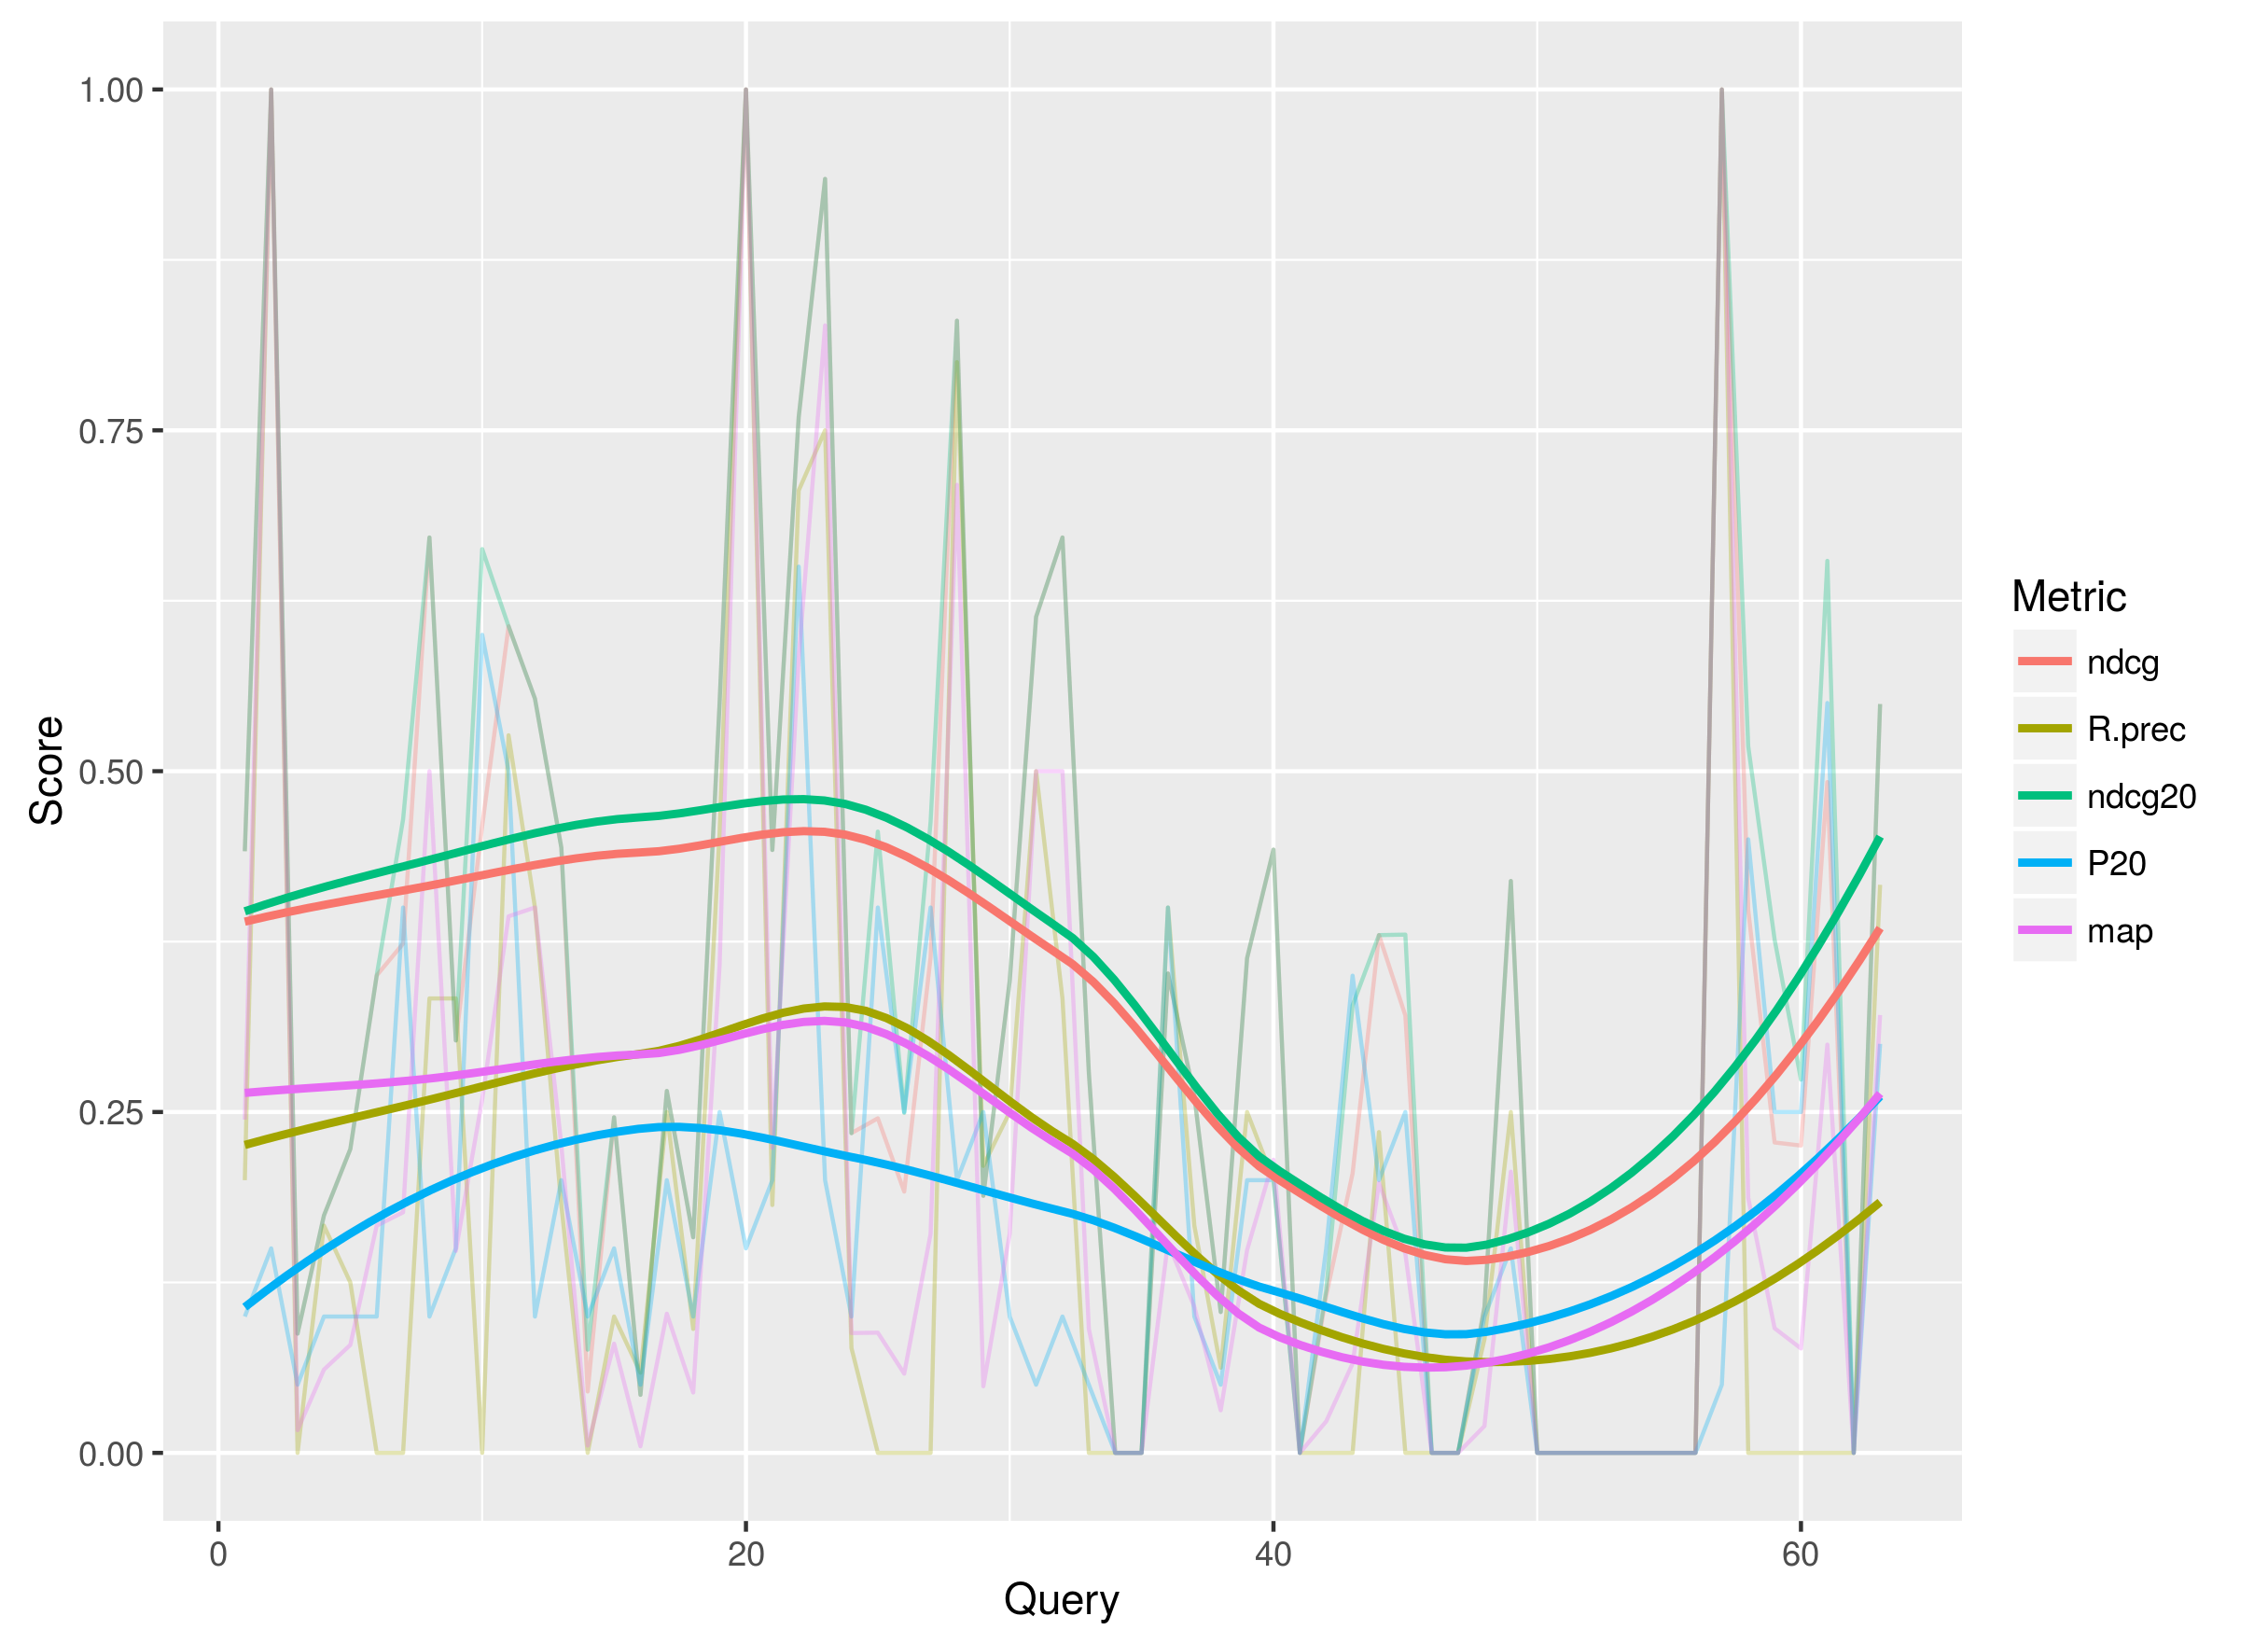
\includegraphics[scale=0.7]{q3_plot_r20.png}
\caption{R-precision Comparison r=20} 
\label{fig:q3plot_r20}
\end{figure}
At r=20, \autoref{fig:q3plot_r20}, the R-Precision increases to be on par with MAP and the P20 is mirrored in compairison to \autoref{fig:q3plot}. The ndcg20 value is greater than the overall ndcg for all queries which would be expected but why that is so will at the end of this section. At r=100, \autoref{fig:q3plot_r100}, R-Precision and MAP show only a marginal increase but NDGC100 has the largest increase overall whereas P100 is almost 0. 
\begin{figure}[H]
\centering
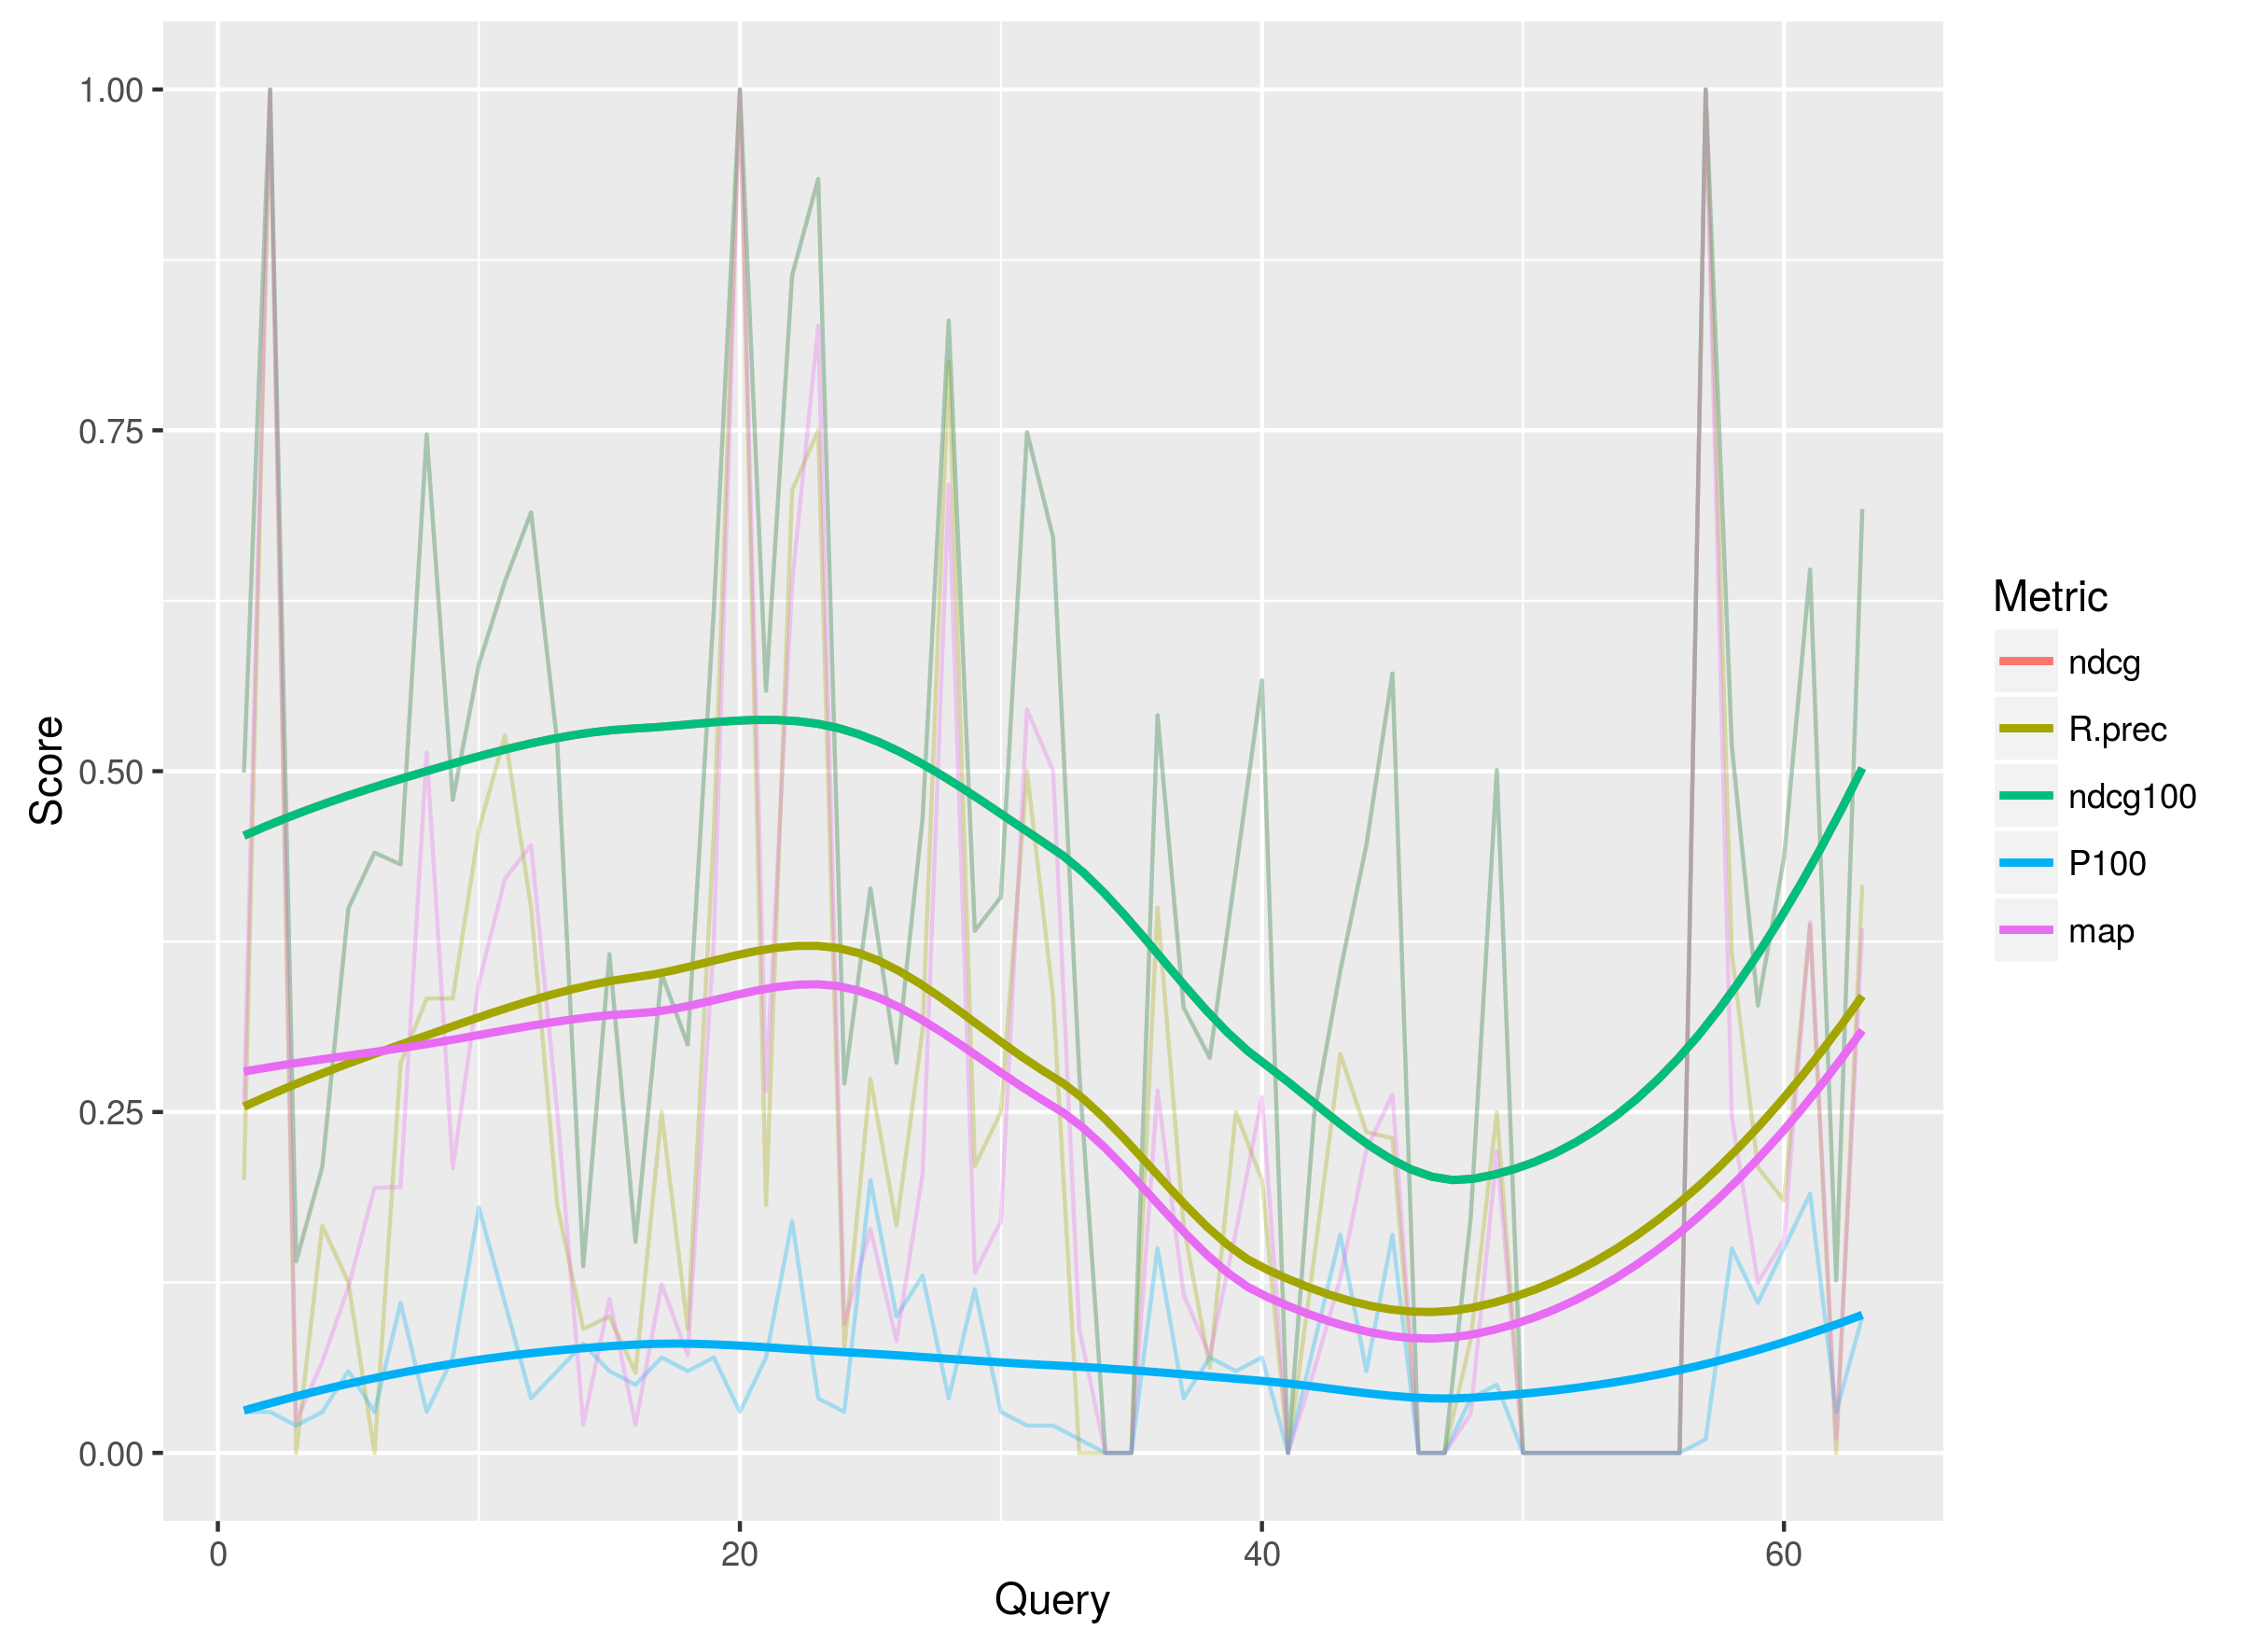
\includegraphics[scale=0.7]{q3_plot_r100.png}
\caption{R-precision Comparison r=100}
\label{fig:q3plot_r100}
\end{figure}
The only explanation for this can be found in the number of relevant documents greater than or equal to ten according to the \textit{cam.rel} file. \autoref{tbl:gt10} shows these numbers and from the previous discussion about how galago computes these metrics it is clear to see that all relevant documents are taken into consideration for these scores. 
\begin{table}[H]
\caption{Relevant Document $>=$ 10 Count }
\begin{minipage}{.5\linewidth}
\centering
       \begin{tabular}{rr}
  \hline
 Query & Count \\ 
  \hline
4 &  12 \\ 
   7 &  28 \\ 
  10 &  35 \\ 
  11 &  19 \\ 
  13 &  11 \\ 
  14 &  44 \\ 
  15 &  10 \\ 
  16 &  17 \\ 
  17 &  16 \\ 
  18 &  11 \\ 
  19 &  11 \\ 
  21 &  11 \\ 
  22 &  17 \\ 
  24 &  13 \\ 
  25 &  51 \\ 
  26 &  30 \\ 
  27 &  29 \\ 
   \hline
\end{tabular}
    \end{minipage}%
    \centering
    \begin{minipage}{.5\linewidth}
       \begin{tabular}{rr}
  \hline
 Query & Count \\ 
  \hline
    29 &  19 \\ 
  36 &  20 \\ 
  37 &  12 \\ 
 38 &  16 \\ 
  39 &  12 \\ 
  40 &  10 \\ 
  42 &  21 \\ 
  43 &  41 \\ 
  44 &  17 \\ 
  45 &  26 \\ 
  48 &  12 \\ 
  58 &  30 \\ 
  59 &  43 \\ 
  60 &  27 \\ 
  61 &  31 \\ 
  63 &  12 \\ 
   \hline
\end{tabular}
    \end{minipage} 
\label{tbl:gt10}
\end{table}

\begin{code}
\captionof{listing}{Plot data Gen} 
\label{code:q3}
	\pycode{code/q3_8.7.py}
\end{code}
\begin{code}
\captionof{listing}{Plot Generator} 
\label{code:q3p}
	\rcode{code/q3_plotter.R}
\end{code}
\newpage
\section{Question 9.6} \label{q4}
\begin{verbatim}
Compare the accuracy of a one versus all SVM classifier and a one versus
one SVM classifier on a multiclass classification data set. Discuss any differences
observed in terms of the efficiency and effectiveness of the two approaches.
\end{verbatim}
\subsection{Answer} 
This questions answer follows the example for SVMs on scikit-learns \href{http://scikit-learn.org/stable/auto_examples/svm/plot_iris.html}{website} as it provides a python interface for both liblinear and libsvm. Dataset used is the publicly available iris dataset which comes packaged with sciki-learn. The code used for this question can be seen in \autoref{code:q4} and uses two different linear SVM implementations SVC(libsvm) and LinearSVC(liblinear). The SVC or SVM class C utilizes a one-vs-one for multiclass and LinearSVC a one-vs-all for multiclass. Also in order to ensure these svm implementations did the correct one-vs-one and one-vs-all classification on the iris dataset they were wrapped in a multiclass classification strategy helper  for the respective one-vs-x classification. \newline \newline
\autoref{fig:q5svms} shows the partitioning done by the classifiers on the iris dataset where the color represent the iris type. The one-vs-one strategy created partitions that encompassed the iris types evenly whereas the one-vs-all strategy took more from the light blue iris type. Also one-vs-all did not include the single dark blue iris type in its true class rather classified it as light blue.
\begin{figure}[H]
\centering
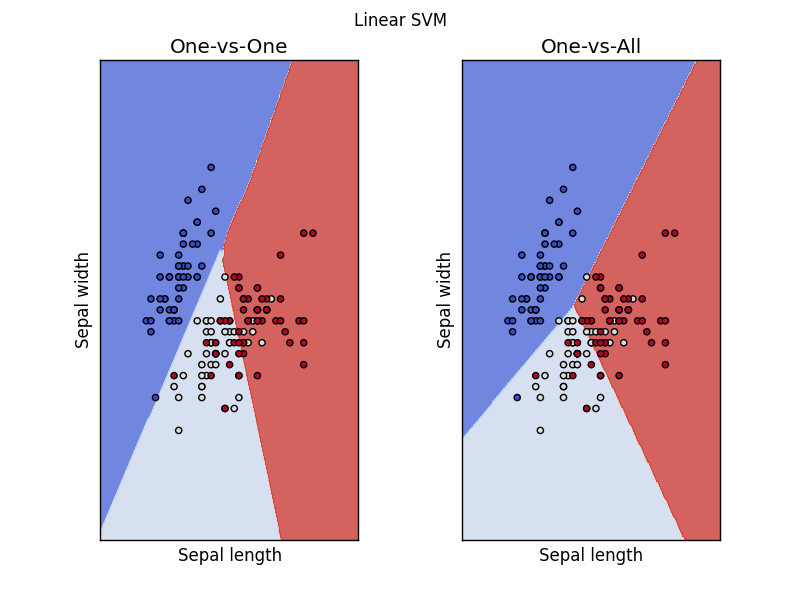
\includegraphics[scale=.7]{svm_linear_1v1_1va.png}
\caption{1v1 and 1vAll Classification Comparison}
\label{fig:q5svms}
\end{figure}
 \autoref{fig:svm_cm}  shows the confusion matrix for the one-vs-one strategy and the color represents the number of iris types classified for a label. As shown in the confusion matrices the one vs one strategy did marginally better than the one vs all strategy for versicolor. \autoref{tbl:ovo} which shows the classification report for one-vs-one and \autoref{tbl:ova} shows the classification report for one-vs-all also reflect that one-vs-one performed better. The support for both strategies are the same which leads me to conclude that using one-vs-one vs one-vs-all depends on the classification task at hand. This toy example highlighted the one-vs-one performance gains as the iris types are distributed close together for the outliers that when using the one-vs-all  strategy it would  pick up on this and wrongly classify iris types when they are extremely close together.

\begin{figure}[H]
\centering
\hspace*{-2cm} 
\begin{subfigure}{.5\textwidth}
  \centering
  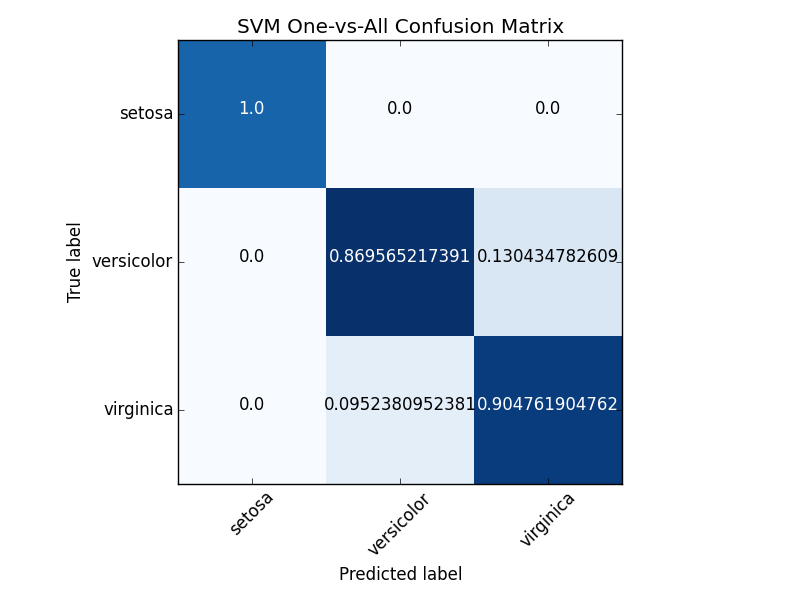
\includegraphics[width=1.2\linewidth]{svm_linear_1va_cm.png}
   \label{fig:sub1}
\end{subfigure}%
\begin{subfigure}{.5\textwidth}
  \centering
  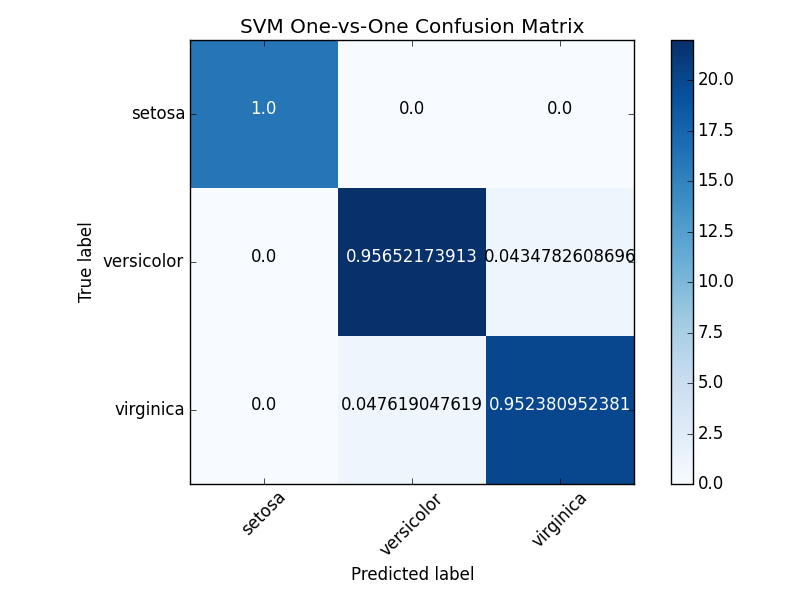
\includegraphics[width=1.2\linewidth]{svm_linear_1v1_cm.png}
   \label{fig:sub2}
\end{subfigure}
\caption{Classification Strategy Confusion Matrices}
\label{fig:svm_cm}
\end{figure}

\begin{table}[H]
\centering
\begin{tabular}{c | c c c c}
Class & Precision & Recall & F-score & Support\\
\hline
\hline\\
setosa & 1.0 & 1.0 & 1.0 & 16\\
versicolor & 0.96 & 0.96 & 0.96 & 23\\
virginica & 0.95 & 0.95 & 0.95 & 21\\
avg & 0.97 & 0.97 & 0.97 & 60\\
\end{tabular}
\caption{Classification Report for One-vs-One}
\label{tbl:ovo}
\end{table}
\begin{table}[H]
\centering
\begin{tabular}{c | c c c c}
Class & Precision & Recall & F-score & Support\\
\hline
\hline\\
setosa & 1.0 & 1.0 & 1.0 & 16\\
versicolor & 0.91 & 0.87 & 0.89 & 23\\
virginica & 0.86 & 0.9 & 0.88 & 21\\
avg & 0.92 & 0.92 & 0.92 & 60\\
\end{tabular}
\caption{Classification Report for One-vs-All}
\label{tbl:ova}
\end{table}
\begin{code}
\captionof{listing}{svm code} 
\label{code:q4}
	\pycode{code/q4_9.6.py}
\end{code}
\newpage
\section{Question 9.8} \label{q5}
\begin{verbatim}
Use K-means and spherical K-means to cluster the data points in Exercise
9.8. How do the clusterings differ?
\end{verbatim}
\subsection{Answer} 
Scikit learn was also used to answer this question as well as an extension of its kmeans class SphericalKMeans provided by spherecluster which extends scikit learns version to do the sphericalkmeans. 
The points from $9.8$ are $(-4, -2), (-3, -2), (-2, -2), (-1, -2), (1, -1), (1, 1), (2, 3), (3, 2), (3, 4), (4, 3)$ and the code used to answer this question can be seen in \autoref{code:q5}.  The k value chosen was 3 due to the sparse nature of the points which can be seen in \autoref{fig:q5plot}. \autoref{fig:kmeansiter} which shows the kmeans algorithm after the first iteration and \autoref{fig:kmeansfull} shows the kmeans algorithm after running to completion. The biggest difference seen in \autoref{fig:q5plot} is how the centroids are placed even after the first iteration. Kmeans drops the points directly in the middle of the clusters whereas sphericalkmeans puts them in the middle and works outwards in a spiral.  I believe this is happening due to the n\_init parameter which runs the algorithm with n different initial seeds after which it chooses the best.

\begin{figure}[H]
\centering
\hspace*{-3cm} 
\begin{subfigure}{.5\textwidth}
  \centering
  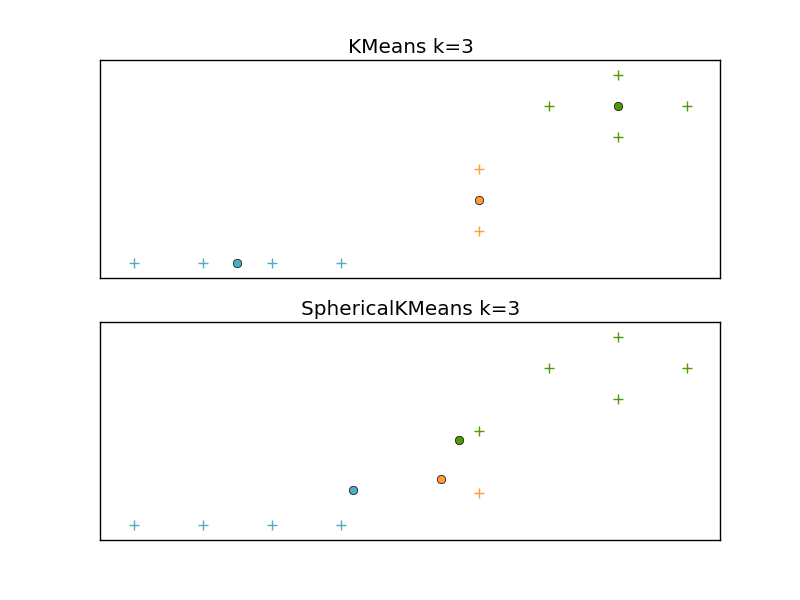
\includegraphics[width=1.2\linewidth]{kmeans_vs_sphericalkmean_iter.png}
   \caption{One Iteration}
   \label{fig:kmeansiter}
\end{subfigure}%
\hspace*{1cm} 
\begin{subfigure}{.5\textwidth}
  \centering
  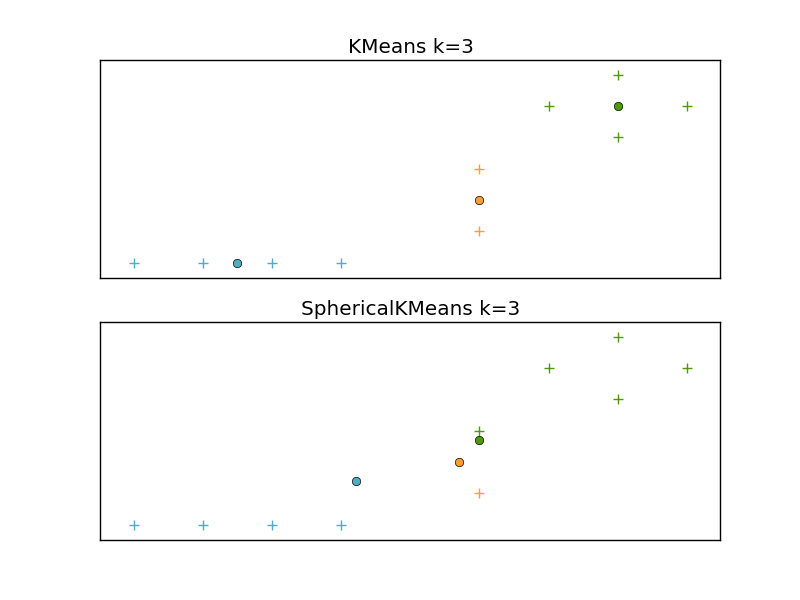
\includegraphics[width=1.2\linewidth]{kmeans_vs_sphericalkmean.png}
  \caption{Run To Completion}
   \label{fig:kmeansfull}
\end{subfigure}
\vspace{1cm}
\caption{Classification Strategy Confusion Matrices}
\label{fig:q5plot}
\end{figure}

\begin{code}
\captionof{listing}{kmeans code} 
\label{code:q5}
	\pycode{code/q5_9.8.py}
\end{code}
\newpage
\begin{code}
\captionof{listing}{Ranking methods found on gist} 
\label{code:q1rnk}
	\pycode{code/ranking_methods.py}
\end{code}
\newpage
\begin{code}
\captionof{listing}{Context Helper Classes} 
\label{code:cntx}
	\pycode{code/contextClasses.py}
\end{code}
\newpage
\begin{code}
\captionof{listing}{CACM Helper Functions} 
\label{code:cacm_help}
	\pycode{code/cam_q_utils.py}
\end{code}

\begin{code}
\captionof{listing}{General Utility Functions} 
\label{code:util}
	\pycode{code/util.py}
\end{code}
\begin{code}
\captionof{listing}{Run Galago Bash File} 
\label{code:rungal}
	\shellcode{rungalago.sh}
\end{code}
\end{document}